\documentclass[../final_report.tex]{subfiles}
\usepackage{subfiles}
\usepackage{diagbox}
\graphicspath{{../../Lab4/plots/}}
\begin{document}

Σκοπός της συγκεκριμένης άσκησης είναι η μελέτη και η αξιολόγηση της επίδοσης μιας ταυτόχρονης
δομής δεδομένων. Η δομή αυτή είναι μια απλά συνδεδεμένη ταξινομημένη λίστα. Εκτελώντας πειράματα,
βγαίνουμε σε συμπεράσματα για το πως οι διαφορετικοί τρόποι συγχρονισμού αποφέρουν και διαφορετικά
αποτελέσματα. 

\subsubsection*{Δομή Συνδεδεμένης Λίστας}
Οι δομές της απλά συνδεδεμένης λίστας είναι:

\begin{lstlisting}
    typedef struct ll_node {
        int key;
        struct ll_node *next;
    } ll_node_t;
    
    struct linked_list {
        ll_node_t *head;
    };    
\end{lstlisting}

Ένα set αποτελείται από μια συνδεδεμένη λίστα κόμβων (linked list of nodes). Το περιεχόμενο του κόμβου το αγνωούμε καθώς
δεν επηρεάζει τις μετρήσεις μας. Το αναγνωριστικό του κάθε κόμβου είναι ο αριθμός key. Ο πρώτος και ο τελευταίος κόμβος έχουν
ιδιαίτερη σημασία και ονομάζονται head και tail αντίστοιχα. Ακολουθούμε τις εξής συμβάσεις για τα πειράματά μας:

\begin{itemize}
    \item Τα head, tail nodes είναι σταθερά, δεν αφαιρούνται ούτε προστίθονται. Αποκαλούνται sentinel nodes.
    \item Η λίστα είναι ταξινομημένη βάσει κλειδιού, τα κλειδία είναι unique.
    \item Οι παρακάτω μέθοδοι ακολουθούν τους 2 αυτούς κανόνες. Π.χ. η μέθοδος add() δεν θα προσθέσει κόμβο με κλειδί ίδιο με ήδη υπάρχοντα κόμβο.
    \item Ένα αντικείμενο ανήκει στην λίστα μόνο και μόνο αν υπάρχει μονοπάτι που το βρίσκει έχοντας ως αφετηρία τον κόμβο head.
\end{itemize}

Οι μέθοδοι που υποστηρίζονται από αυτή την δομή είναι: 

\begin{itemize}
    \item \textbf{contains(x):} Επιστρέφει True μόνο και μόνο αν η λίστα περιέχει το x.
    \item \textbf{add(x):} Προσθέτει το x στην λίστα και επιστρέφει True μόνο αν το x δεν υπήρχε ήδη στην λίστα.
    \item \textbf{remove(x):} Αφαιρεί το x από την λίστα και επιστρέφει True μονο αν το x υπήρχε στην λίστα (και διαγράφηκε).
\end{itemize}

Μελετάμε την συμπεριφορά των παρακάτω τρόπων συγχρονισμού για διαφορετικό αριθμό νημάτων \{1, 2, 4, 8, 16, 32, 64, 128\},
για διαφορετικό μέγεθος λίστας \{1024, 8192\} και για διαφορετικό ποσοστό λειτουργιών \{100/0/0, 80/10/10, 20/40/40, 0/50/50\}.
Για το ποσοστό λειτουργιών, ο πρώτος αριθμός δηλώνει ποσοστό αναζητήσεων, ο δεύτερος εισαγωγών και ο τρίτος διαγραφών.

\subsubsection*{Επεξήγηση των Workloads}
Είναι πολύ πιο ρεαλιστικό σε μια εφαρμογή να υπάρχουν περισσότερες κλήσεις τις μεθόδου contains() παρά των add() και remove().
Τα πρώτα 2 ενδεχόμενα καλύπτουν αυτές τις ρεαλιστικές χρήσεις. Τα workloads 20/40/40 και 0/50/50 είναι πιο ακραία και πιο σπάνια
σε κλασσικές εφαρμογές.

\subsubsection*{Serial}

Η σειριακή εκτέλεση προσφέρεται μόνο για λόγους benchmarking. Μέσω αυτών των αποτελεσμάτων, κρίνουμε και τις υπόλοιπες υλοποιήσεις.
Οι μετρήσεις στον πίνακα αφορούν Throughput, δηλαδή πόσα Operations έκανε η κάθε υλοποίηση σε ένα δευτερόλεπτο. Συγκεκριμένα, ο αριθμός
εκφράζει Kops/sec (Kilo-operations/second).

\noindent
\begin{tabular}{|l||*{4}{c|}}\hline
\backslashbox{Size}{Workload}
&\makebox[3.5em]{100/0/0}&\makebox[3.5em]{80/10/10}&\makebox[3.5em]{20/40/40}
&\makebox[3.5em]{0/50/50}\\\hline\hline
1024 & 1566.15 & 1897.13 & 1612.85 & 1410.06\\\hline
8192 & 151.82 & 69.55 & 81.33 & 65.60\\\hline
\end{tabular}

\subsubsection*{Concurrent Linked List}
Έχοντας δει scalable spin locks στην προηγούμενη άσκηση, τα χρησιμοποιούμε για να επιχειρήσουμε να δημιουργήσουμε
scalable ταυτόχρονες δομές δεδομένων. Το lock που χρησιμοποιούμε σε όλες τις υλοποιήσεις που χρησιμοποιούν lock, είναι
το pthread Spinlock. 

Γνωρίζοντας τα αποτελέσματα από πριν, για να είναι πιο καθαρά τα διαγράμματα, χωρίζουμε τους τύπους του κλειδώματος σε 
low και all performers. Οι μετρικές που χρησιμοποιούμε για να δούμε ποια υλοποίηση είναι καλύτερη είναι το Throughput και το "Speedup".

Εδώ, δεν αναφερόμαστε στον χρόνο, άρα ο ορισμός του Speedup είναι διαφορετικός. Για να δούμε πόσο καλύτερη (ή χειρότερη!) είναι η παράλληλη υλοποίηση από
την σειριακή, χρησιμοποιούμε τον τύπο \(Speedup=\frac{Throughput(Parallel)}{Throughput(Serial)}\). 

Για κάθε τύπο συγχρονισμού, επεξηγούμε το πως πετυχαίνουμε την παράλληλη εκτέλεση και πως εκτελούνται οι 3 προαναφερόμενοι μέθοδοι.

\subsection{Low Performers}
Οι υλοποιήσεις που θεωρούμε "Low Performers" είναι οι παρακάτω. Ο λόγος που τους θεωρούμε χαμηλών επιδόσεων είναι γιατί οι υλοποιήσεις
αυτές είναι απλοϊκές και έχουν ξεκάθαρα προβλήματα που εμφανίζονται στο θεωρητικό επίπεδο. Με βάση αυτά τα προβλήματα,
γνωρίζουμε από πριν την ανικανότητά τους να κλιμακώσουν.

\subsubsection{Coarse-grain Locking}
Η απλούστερη προσπάθεια για ταυτόχρονη συνδεδεμένη λίστα. Υπάρχει ένα lock για όλη την δομή και κάθε φορά που ένα
νήμα θέλει να εφαρμόσει μια μέθοδο, περιμένει μέχρι να αποκτήσει το lock και μετά εκτελεί την λειτουργία του κανονικά.
Η μόνη προσθήκη που πρέπει να κάνουμε στην δομή είναι ένα spinlock και η κάθε μέθοδος να κάνει lock στο κάλεσμά της και 
unlock στο τέλος της.

Το προφανές συμπέρασμα είναι ότι αν και η τεχνική αυτή λειτουργεί πλήρως, η απόδοσή της είναι πάντα όσο η σειριακή ή και
χειρότερη λόγω του overhead του κλειδώματος. 

\subsubsection{Fine-grain Locking}
Εφόσον η συνδεδεμένη λίστα αποτελείται από ένα πεπερασμένο πλήθος κόμβων, μπορούμε αντί να έχουμε ένα lock για όλη την δομή,
να έχουμε πολλαπλά locks, συγκεκριμένα ένα για κάθε κόμβο. Αυτό το καταφέρνουμε τοποθετώντας ένα spinlock σε κάθε node της συνδεδεμένης λίστας.

Πλέον, για να υπάρχει ασφάλεια στην χρήση των μεθόδων από τα νήματα, πρέπει να υπάρξει ένα σύστημα hand-over-hand locking. 
Για να κλειδώσει ο curr κόμβος πρέπει να είναι ήδη κλειδωμένος ο pred κόμβος. Αυτό το κλείδωμα και ξεκλείδωμα πρέπει πάντα να γίνεται
με αυτή την ακολουθία.
\begin{figure}[H]
    \centering
        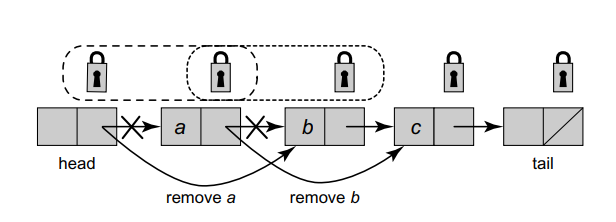
\includegraphics[scale=0.7]{fglRemove.png}
    \caption{Fine-grained Locking - Remove method - Hand-over-Hand locking}
    \label{fig:Fine-grained Locking - Remove method - Hand-over-Hand locking}
\end{figure}

Για την διαγραφή, πρέπει να κλειδωθεί ο κόμβος που πρόκεται να κλειδωθεί για να μην δράσει κάποια άλλη λειτουργία πάνω του και επίσης
πρέπει να κλειδωθεί ο προηγούμενος κόμβος καθώς αυτός θα πραγματοποιήσει την διαγραφή, αλλάζοντας την διεύθυνση next.

Η διάσχιση της λίστας πρέπει αποκλειστικά να γίνεται με αυτό το σύστημα lock coupling. Συνέπεια αυτόυ είναι ότι αν ένα στοιχείο κλειδώσει
στις αρχές της λίστας, απαγορεύεται από άλλα νήματα να επεξεργαστούν αργότερα στοιχεία που βρίσκονται πιο μετά στην λίστα.

Το fine-grained locking μπορεί να δεχτεί πολλές βελτιώσεις. Είναι πολύ πιθανό κάποια νήματα να περιμένουν πολύ
ώρα να αποκτήσουν πρόσβαση στην δομή σε τελείως διαφορετικά σημεία από αυτά που επεξεργάζονται άλλα νήματα.
Για αυτό ευθύνεται η ανάγκη για hand-over-hand locking.

\subsubsection{Optimistic synchronization}
Στην "αισιόδοξη" υλοποίηση, περιμένουμε να έχουμε πολύ μικρές πιθανότητες κάτι να πάει στραβά. Αναζητούμε χωρίς να 
κλειδώνουμε τα στοιχεία αλλά με το που βρούμε τους κόμβους που μας ενδιαφέρουν τότε να επαληθεύουμε ότι οι κλειδωμένοι
κόμβοι είναι οι σωστοί. Αν λόγω κακού συγχρονισμού κλειδώνουμε τους λάθους κόμβους, τότε απελευθερώνουμε τις κλειδαριές και
ξαναπροσπαθούμε.

Άρα, αποδεχόμαστε το ρίσκο αλλά δεν αφήνουμε την δομή πλήρως ασυνεπή. Προσθέτουμε την μέθοδο \textbf{validate()}. 
Η μέθοδος αυτή ελέγχει αν τα δύο στοιχεία (pred,curr) βρίσκονται ακόμα στην δομή. 
Με βάση τις παραπάνω συμβάσεις αυτό σημαίνει:

\begin{itemize}
    \item O pred κόμβος να είναι προβιβάσιμος από το head της δομής
    \item Να ισχύει (pred.next == curr, δηλαδή ο επόμενος του προηγούμενου είναι ο τρέχοντας)
\end{itemize}

Πλέον, για να τρέξουμε τις μεθόδους, ακολουθούμε την εξής λογική:

Δεν κλειδώνουμε όσο διατρέχουμε την λίστα. Όταν φτάσουμε στο σημείο που θέλουμε να εκτελέσουμε ενέργεια, τότε κλειδώνουμε
τον προηγούμενο ακριβώς κόμβο και τον κόμβο που θέλουμε να εκτελέσουμε ενέργεια. Αφού γίνει το κλείδωμα, τρέχουμε την validate(pred, curr).
Αν αποτύχει, ξαναξεκινάμε την διαδικασία. Αν πετύχει, εκτελούμε την ενέργεια που θέλαμε. Τέλος, ξεκλειδώνουμε πάλι με την ίδια σειρά, πρώτα 
τον προηγούμενο κόμβο και μετά τον τωρινό. 

\begin{figure}[H]
    \centering
        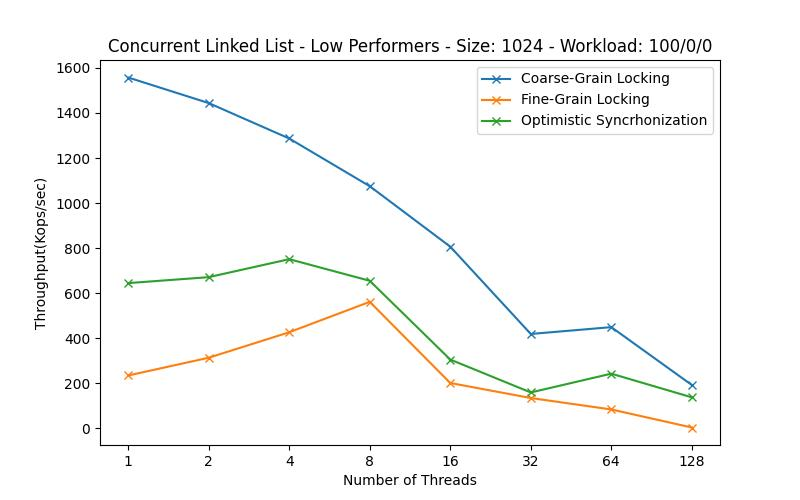
\includegraphics[scale=0.4]{outFiles/plots/concurrent_data_structs_low_1024_100_0_0.jpg}
        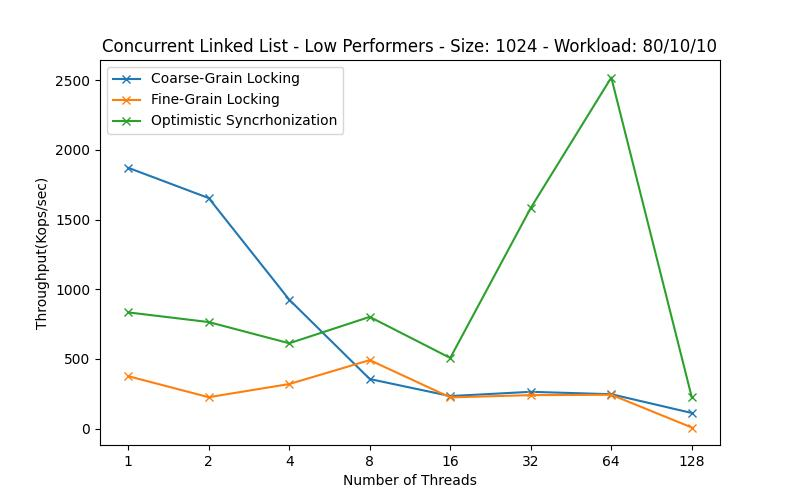
\includegraphics[scale=0.4]{outFiles/plots/concurrent_data_structs_low_1024_80_10_10.jpg}
        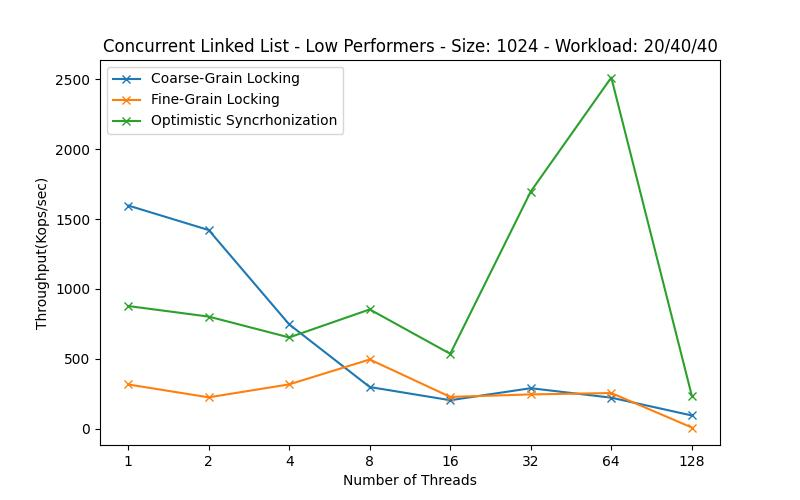
\includegraphics[scale=0.4]{outFiles/plots/concurrent_data_structs_low_1024_20_40_40.jpg}
        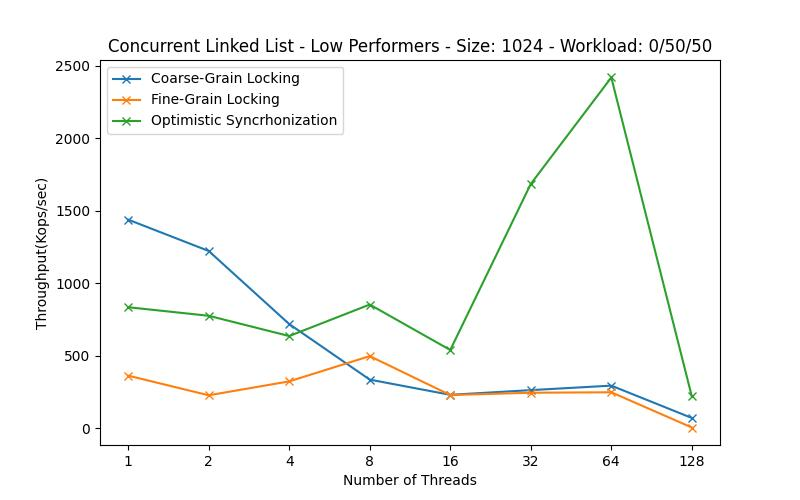
\includegraphics[scale=0.4]{outFiles/plots/concurrent_data_structs_low_1024_0_50_50.jpg}
    \caption{Concurrent Linked List - Throughput - Size 1024 - Low Performers}
    \label{fig:Concurrent Linked List - Throughput - Size 1024 - Low Performers}
\end{figure}

\begin{figure}[H]
    \centering
        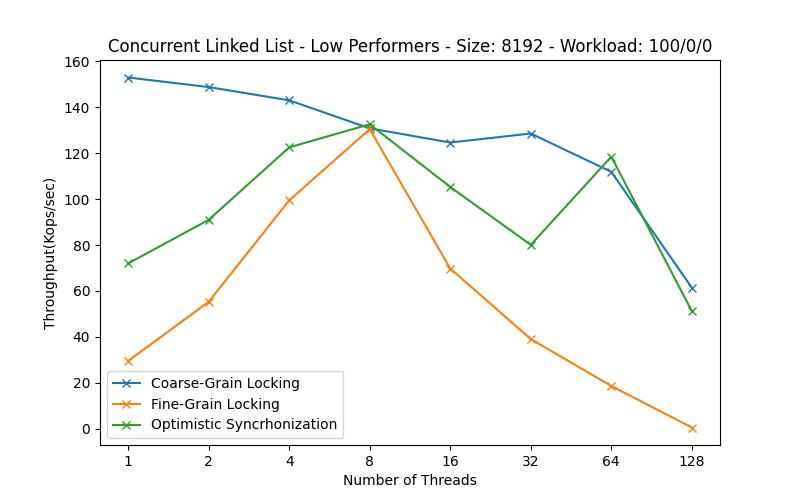
\includegraphics[scale=0.4]{outFiles/plots/concurrent_data_structs_low_8192_100_0_0.jpg}
        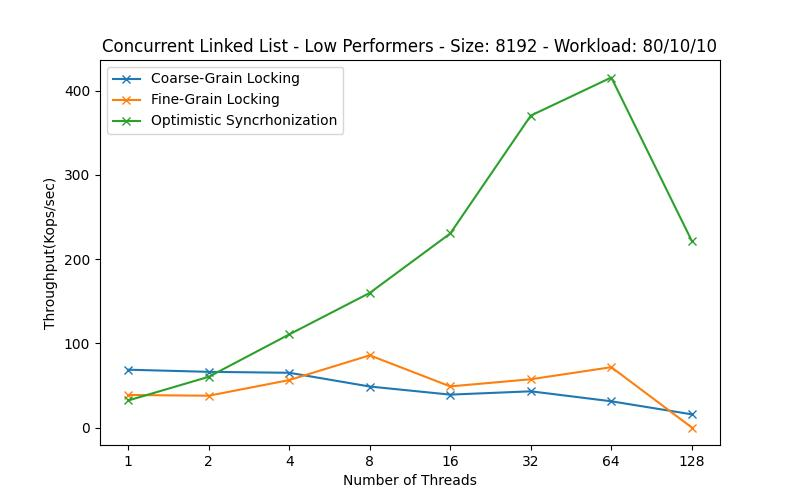
\includegraphics[scale=0.4]{outFiles/plots/concurrent_data_structs_low_8192_80_10_10.jpg}
        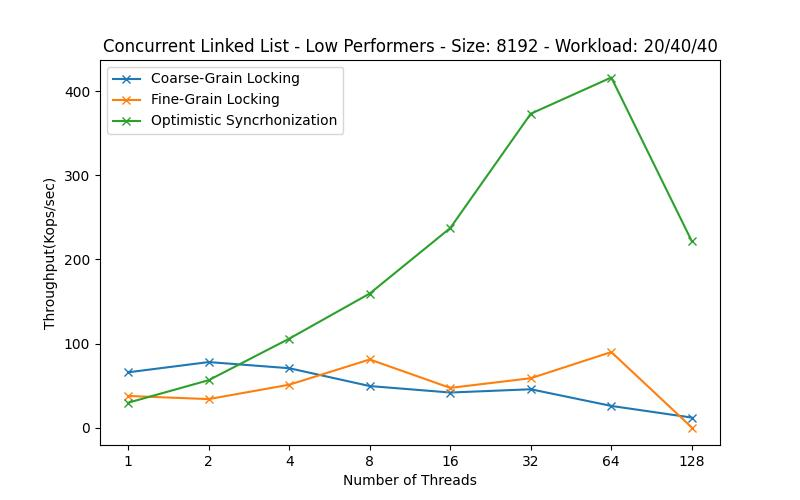
\includegraphics[scale=0.4]{outFiles/plots/concurrent_data_structs_low_8192_20_40_40.jpg}
        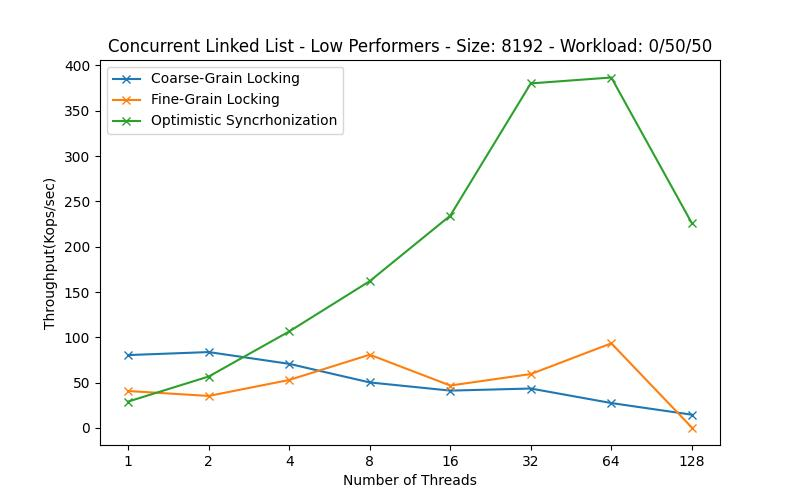
\includegraphics[scale=0.4]{outFiles/plots/concurrent_data_structs_low_8192_0_50_50.jpg}
    \caption{Concurrent Linked List - Throughput - Size 8192 - Low Performers}
    \label{fig:Concurrent Linked List - Throughput - Size 8192 - Low Performers}
\end{figure}

\begin{figure}[H]
    \centering
        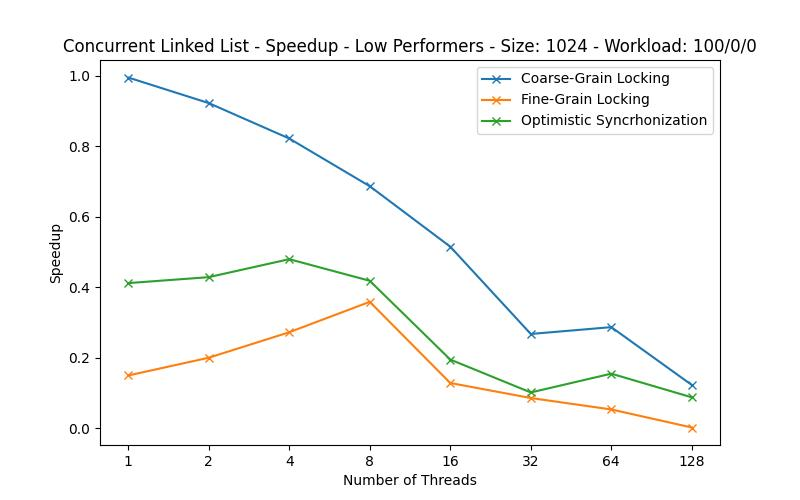
\includegraphics[scale=0.4]{outFiles/plots/concurrent_data_structs_low_speedup_1024_100_0_0.jpg}
        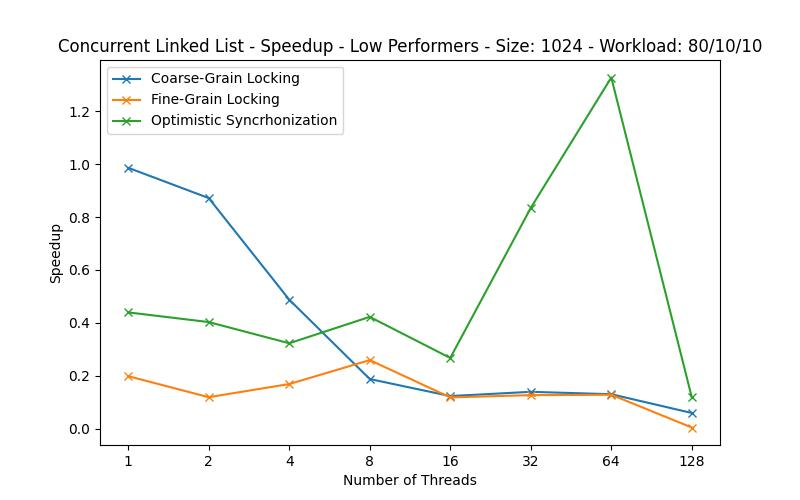
\includegraphics[scale=0.4]{outFiles/plots/concurrent_data_structs_low_speedup_1024_80_10_10.jpg}
        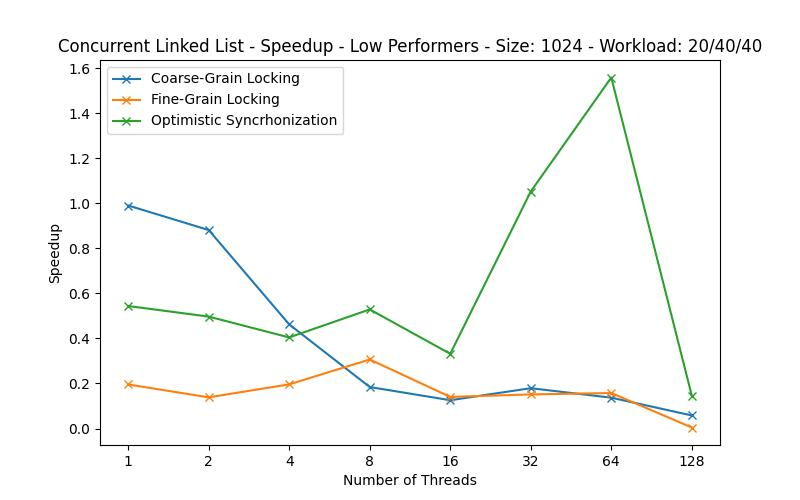
\includegraphics[scale=0.4]{outFiles/plots/concurrent_data_structs_low_speedup_1024_20_40_40.jpg}
        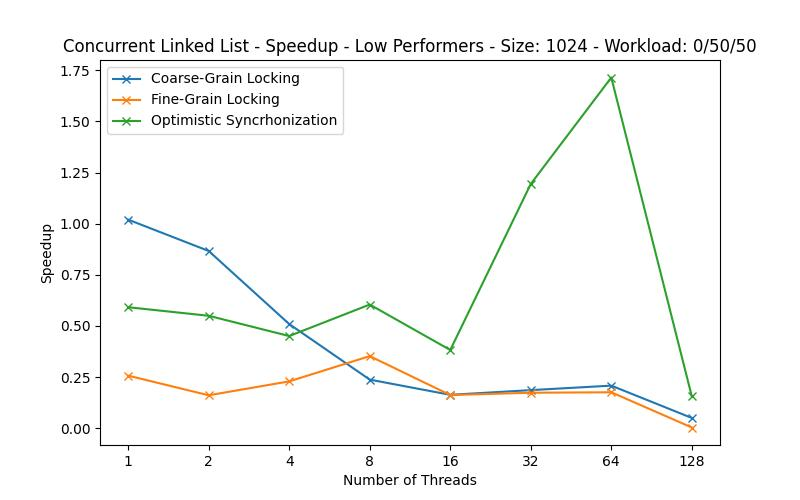
\includegraphics[scale=0.4]{outFiles/plots/concurrent_data_structs_low_speedup_1024_0_50_50.jpg}
    \caption{Concurrent Linked List - Speedup - Size 1024 - Low Performers}
    \label{fig:Concurrent Linked List - Speedup - Size 1024 - Low Performers}
\end{figure}

\begin{figure}[H]
    \centering
        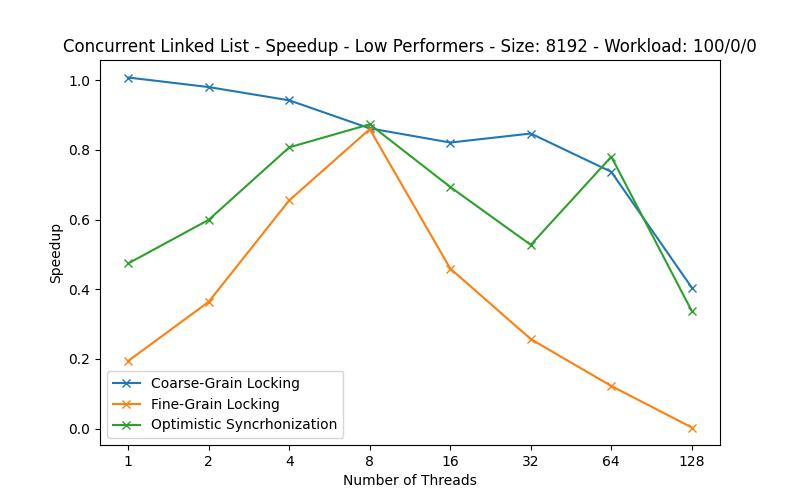
\includegraphics[scale=0.4]{outFiles/plots/concurrent_data_structs_low_speedup_8192_100_0_0.jpg}
        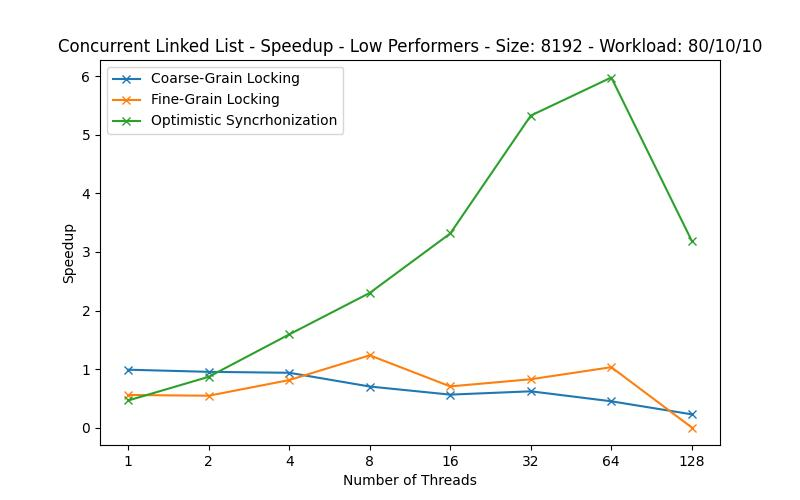
\includegraphics[scale=0.4]{outFiles/plots/concurrent_data_structs_low_speedup_8192_80_10_10.jpg}
        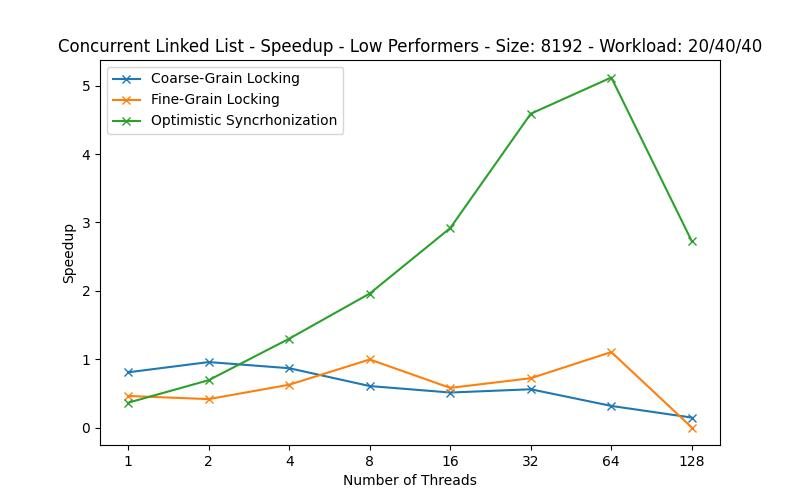
\includegraphics[scale=0.4]{outFiles/plots/concurrent_data_structs_low_speedup_8192_20_40_40.jpg}
        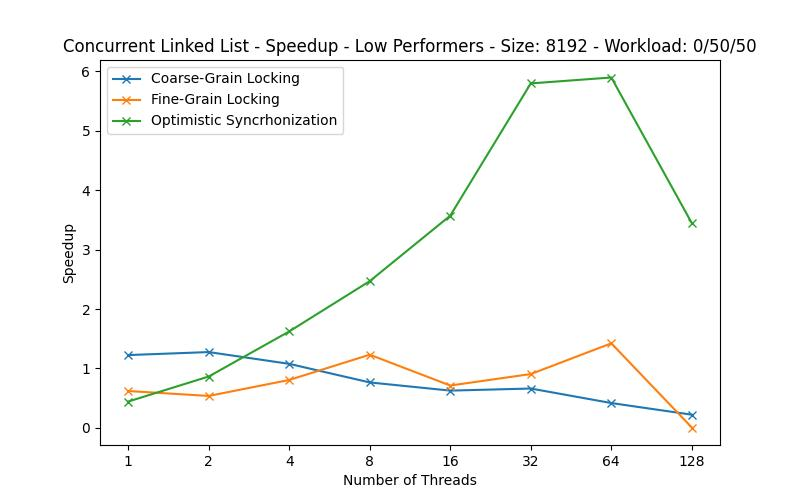
\includegraphics[scale=0.4]{outFiles/plots/concurrent_data_structs_low_speedup_8192_0_50_50.jpg}
    \caption{Concurrent Linked List - Speedup - Size 8192 - Low Performers}
    \label{fig:Concurrent Linked List - Speedup - Size 8192 - Low Performers}
\end{figure}

\subsection*{Low Performers - Συμπεράσματα}

\subsubsection*{Coarse-Grained Synchronization}
Παρατηρώντας τα γραφήματα, βγαίνουμε στο συμπέρασμα ότι για οποιοδήποτε συνδυασμό λειτουργιών ή και
μεγέθους λίστας, η απόδοση του είναι είτε ίση με την σειριακή ή χειρότερη, ανεξαρτήτως workload ή μεγέθους λίστας. Το συμπέρασμα αυτό είναι 
προφανές καθώς η υλοποίηση της coarse-grained λίστας είναι η σειριακή με την προσθήκη ενός lock ώστε
να υπάρχει mutual exclusion μεταξύ νημάτων. 

\subsubsection*{Fine-Grained Synchronization}
Τα συμπεράσματα είναι αρκετά παρόμοια και για την fine-grained υλοποίηση. Οποιαδήποτε λειτουργία απαιτεί να διατρέξουμε
την λίστα από το head της λίστας. Η αναζήτηση αυτή γίνεται πάντα με χρήση του hand-over-hand locking. Δηλαδή, έχουμε πολλαπλά
κλειδώματα και ξεκλειδώματα για οποιαδήποτε λειτουργία. Πάλι, η απόδοση είναι πολύ χειρότερη από την σειριακή ανεξαρτήτως
χαρακτηριστικών μεγέθους/workload.

Σε θέματα ταυτοχρονισμού, η υλοποίηση δεν προσφέρει πολλά. Αν κάποιο νήμα κλειδώσει lock νωρίς στην λίστα, τα υπόλοιπα νήματα
δεν μπορούν να προχωρήσουν μετά από αυτό το σημείο λόγω της αναγκαιότητας για το hand-over-hand locking. 

\subsubsection*{Optimistic Synchronization}
Στην "αισιόδοξη" υλοποίηση παρατηρούμε τις πρώτες βελτιώσεις στην απόδοση. Για μικρές λίστες, απαιτούνται πολλά νήματα, τουλάχιστον 32, ώστε το throughput
να είναι μεγαλύτερο από το σειριακό. Οι επιδόσεις περιορίζονται από το γεγονός ότι η validate() αναγκάζεται να διασχίζει όλη την λίστα μέχρι το σημείο ενδιαφέροντος
και από τα conflicts που μπορεί να προκύπτουν, είτε απόκτησης lock ή synchronization conflict.

Για μεγάλες λίστες, η απόδοση κλιμακώνει αρκετά γραμμικά, μέχρι τα πρώτα 32 νήματα, μετά η επίδοση είτε αυξάνεται ελάχιστα
ή καταρέει. Ενδιαφέρουσα σημείωση ότι η optimistic υλοποίηση δεν έχει καλές επιδόσεις στο workload 100/0/0 αν και η μέθοδος
contains() είναι η πιο "ελαφριά" από τις 3 και θα έπρεπε τουλάχιστον να αποδίδει όπως τα άλλα workloads στην μεγάλη λίστα.

\subsection{High Performers}
Οι υλοποιήσεις που θεωρούμε "High Performers" είναι το lazy και το non-blocking synchronization. Μέχρι στιγμής, η κάθε υλοποίηση προσπαθεί
να διορθώσει τα σημαντικότερα προβλήματα της προηγούμενης. Θα δούμε ότι και οι δύο εκδοχές έχουν πολύ παρόμοιες επιδόσεις.

\subsubsection{Lazy synchronization}
Ο "τεμπέλικος" συγχρονισμός είναι το επόμενο βήμα βελτιστοποίησης. Σε κάθε κόμβο, προσθέτουμε μια boolean τιμή με το όνομα
"marked". Η τιμή αυτή δείχνει αν ένας κόμβος βρίσκεται (λογικά) στην λίστα. Αν η τιμή marked είναι True, τότε ο κόμβος αυτός
έχει αφαιρεθεί λογικά από την λίστα. Ο αλγόριθμος θεωρεί ότι οποιοδήποτε κόμβος δεν είναι marked, είναι και valid στην λίστα.

Η validate() ανανεώνεται ελέγχοντας πλέον και αν κάποιος κόμβος είναι marked. Δεν χρειάζεται να διατρέχει όλη την λίστα.

Πλέον η contains() δεν θα βρεθεί ποτέ σε conflict παρόμοια με αυτά που θα βρισκόταν στην optimistic υλοποίηση,
είναι πλήρως wait-free. Επίσης, η add() και η remove(), αν και κάνουν block, διατρέχουν την λίστα μόνο μια φορά, λόγω της ανανεωμένης validate().
Η add(), διατρέχει την λίστα, κλειδώνει τον predecessor του κόμβου που πρόκεται να προσθέσει, και εκτελεί την ενέργειά της.
Η remove(), πρώτα κάνει mark τον κόμβο που πρόκεται να αφαιρέσει και μετά αλλάζει τον δείκτη του predecessor του στόχου ώστε να έχει
ορθότητα (και συνέχεια) η λίστα.

Την "φυσική" αφαίρεση του κόμβου από την μνήμη την κάνει είτε το σύστημα εκτέλεσης (garbage collector) ή ο προγραμματιστής αν 
γράφει σε κάποια γλώσσα που ο έλεγχος της μνήμης γίνεται χειροκίνητα. Την υλική αυτή αφαίρεση μπορούμε να την κάνουμε ανά batches,
και όχι κάθε φορά που αφαιρούμε λογικά έναν κόμβο, δηλαδή έχουμε έλεγχο για το πότε θα τρέξουμε αυτή την, μπορεί χρονοβόρα, ενέργεια.

Οι βελτιώσεις αυτές καθιστούν την lazy υλοποίηση πολύ ελκυστική λύση. Περιμένουμε να δούμε πολύ καλύτερα αποτελέσματα, ειδικά 
σε workloads που έχουν μεγάλο ποσοστό contains(), καθώς αυτή η μέθοδος είναι πλέον wait-free. 

\subsubsection{Non-blocking synchronization}
Οι τελικές βελτιστοποιήσεις που μπορούμε να κάνουμε είναι να αφαιρέσουμε πλήρως την ανάγκη για locks. Η μέθοδος contains() ήδη λειτουργεί
χωρίς κλειδώματα και δεν χρειάζεται να κάνουμε κάποιες αλλαγές σε αυτή.

Θα προσπεράσουμε αρκετές λεπτομέρειες για το πως λειτουργεί ο non-blocking συγχρονισμός καθώς είναι εξαιρετικά περίπλοκος προγραμματιστικά.

Οι μέθοδοι add() και remove() όμως πρέπει να δεχτούν αλλαγές. Η πρώτη αλλαγή είναι να θεωρήσουμε την διεύθυνση next και την τιμή
marked του κάθε κόμβου ως μια "μονή ατομική μονάδα", δηλαδή, οποιαδήποτε προσπάθεια να αλλάξει η τιμή της next όταν η τιμή marked είναι
True, θα αποτύχει.

Σε αντίθεση με την lazy υλοποίηση που η φυσική αφαίρεση μπορούσε να γίνει σε δική μας κλήση, η non-blocking λίστα ακολουθεί διαφορετική λογική.
Οι add() και remove(), όσο διατρέχουν την λίστα, ελέγχουν για marked κόμβους. Αν βρουν marked κόμβο, εκτελούυν μια μέθοδο compareAndSet(), με σκοπό
την αφαίρεση αυτού του κόμβου. Η συμπεριφορά αυτή είναι κοινή και για τις 2 μεθόδους. Και οι 2 μέθοδοι χρησιμοποιούν ατομική μέθοδο compare-and-swap
για να εκτελέσουν τις ενέργειές τους. Αν για οποιοδήποτε λόγο η remove() δεν καταφέρει να αφαιρέσει φυσικά τον κόμβο, δεν ξαναπροσπαθεί γιατί 
θα επιχειρήσουν και τα επόμενα νήματα όσο διατρέχουν την λίστα.

Με αυτές τις αλλαγές, επιτυχώς υλοποιήσαμε μια λίστα η οποία δεν έχει ανάγκη από lock για να προσφέρει safe concurrency. Η απαλειφή των κλειδαριών
επίσης προσφέρει και μια πιο ανθεκτική δομή η οποία δεν κινδυνεύει από αποτυχία σε ενδεχόμενο "θανάτου" νήματος που κρατάει lock.

\begin{figure}[H]
    \centering
        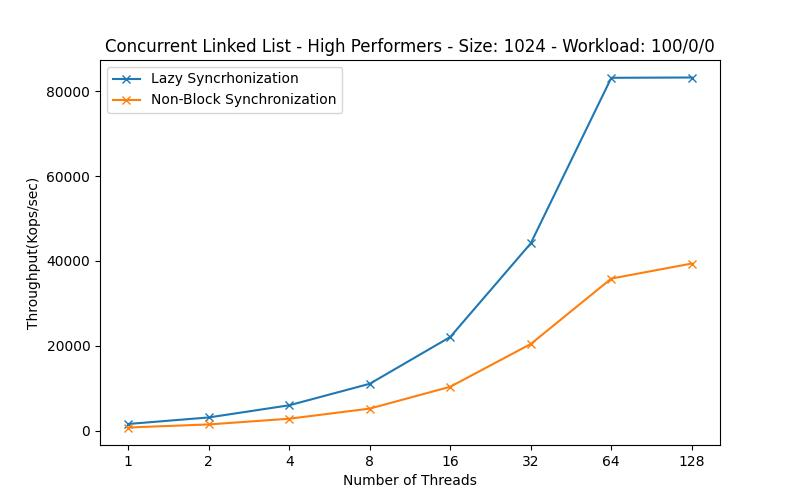
\includegraphics[scale=0.4]{outFiles/plots/concurrent_data_structs_high_1024_100_0_0.jpg}
        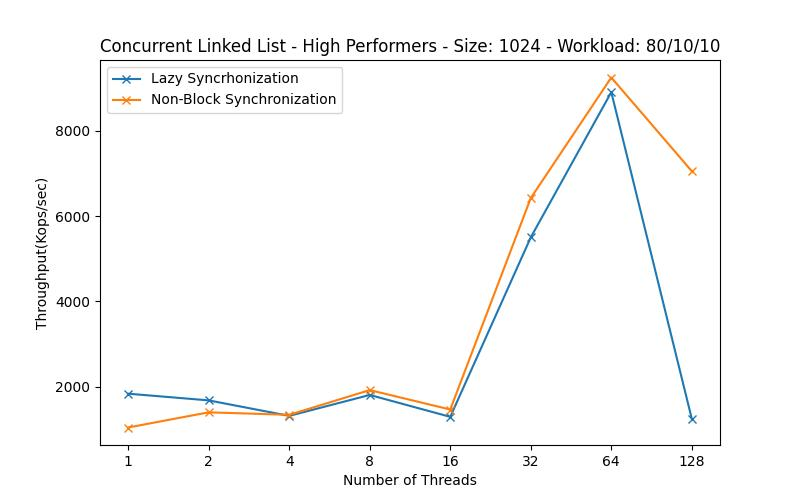
\includegraphics[scale=0.4]{outFiles/plots/concurrent_data_structs_high_1024_80_10_10.jpg}
        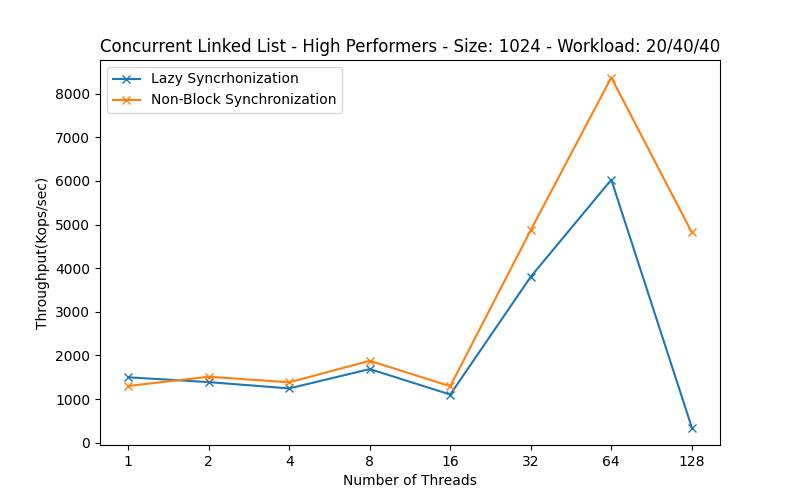
\includegraphics[scale=0.4]{outFiles/plots/concurrent_data_structs_high_1024_20_40_40.jpg}
        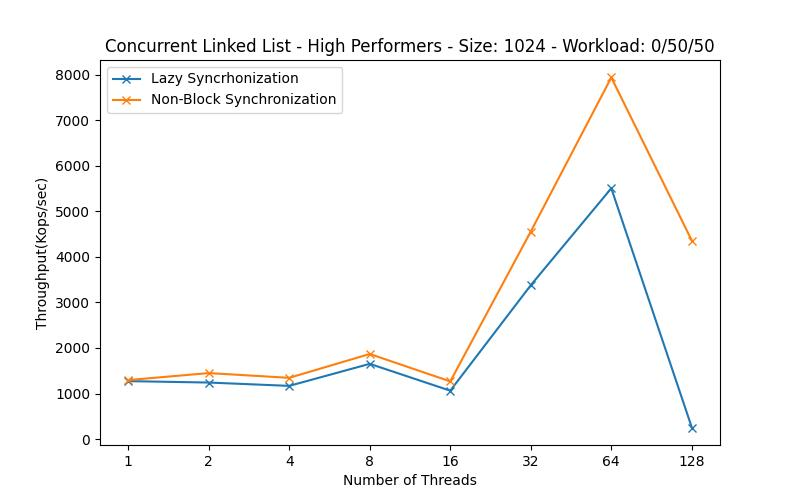
\includegraphics[scale=0.4]{outFiles/plots/concurrent_data_structs_high_1024_0_50_50.jpg}
    \caption{Concurrent Linked List - Throughput - Size 1024 - High Performers}
    \label{fig:Concurrent Linked List - Throughput - Size 1024 - High Performers}
\end{figure}

\begin{figure}[H]
    \centering
        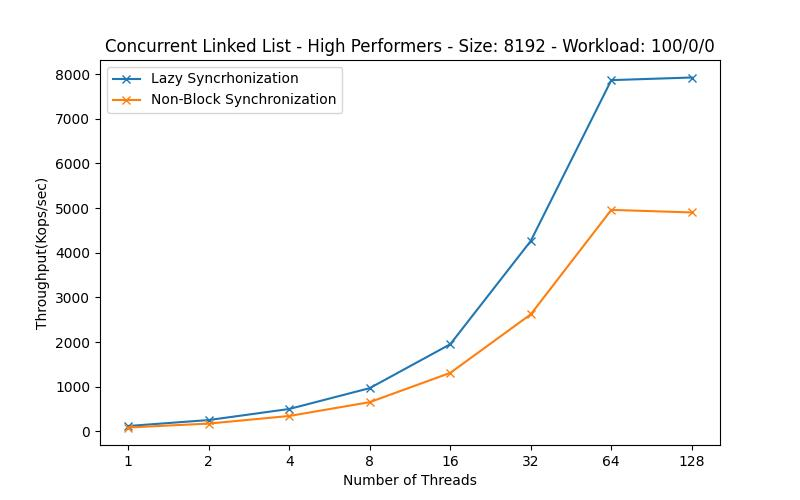
\includegraphics[scale=0.4]{outFiles/plots/concurrent_data_structs_high_8192_100_0_0.jpg}
        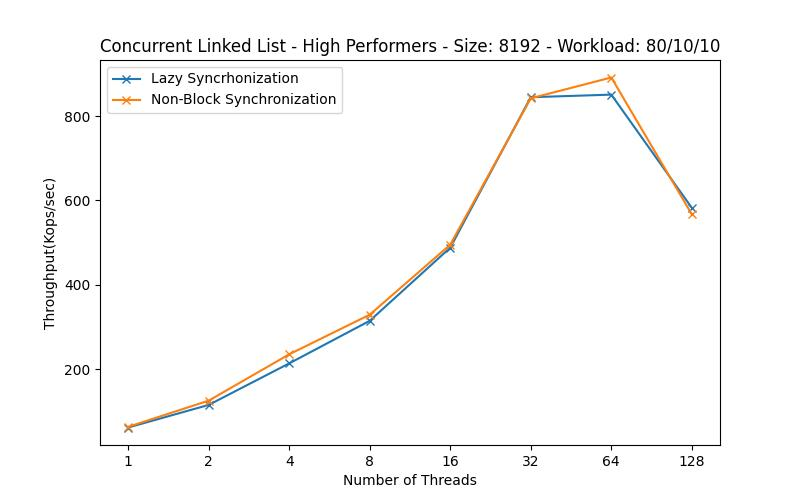
\includegraphics[scale=0.4]{outFiles/plots/concurrent_data_structs_high_8192_80_10_10.jpg}
        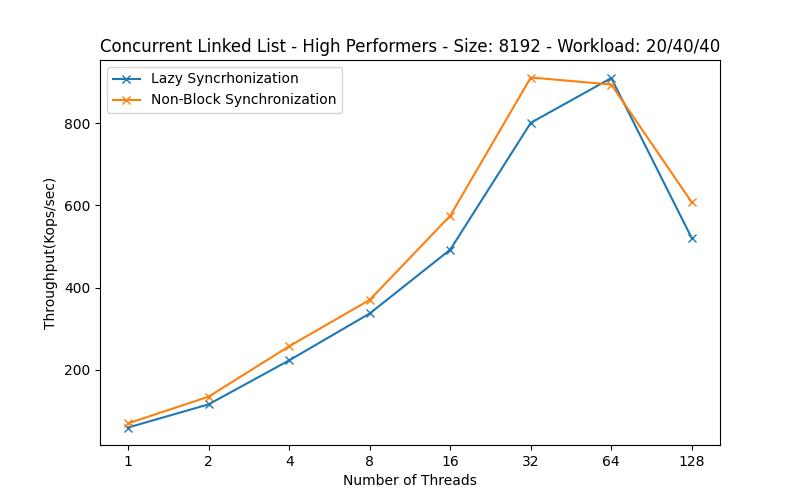
\includegraphics[scale=0.4]{outFiles/plots/concurrent_data_structs_high_8192_20_40_40.jpg}
        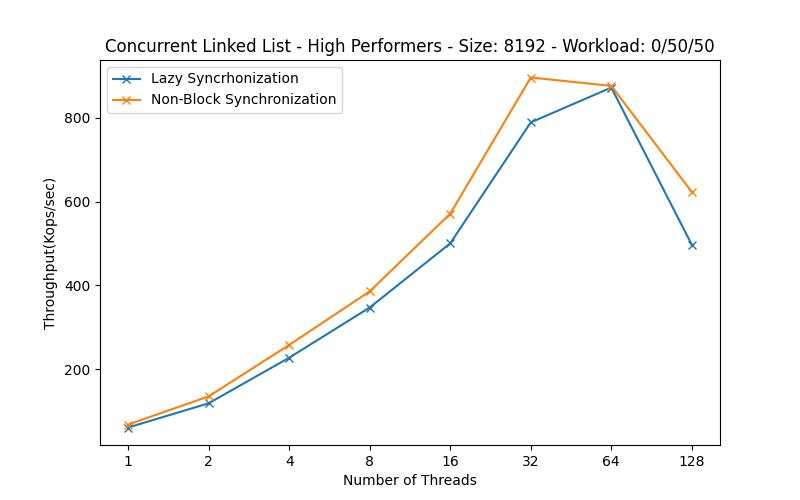
\includegraphics[scale=0.4]{outFiles/plots/concurrent_data_structs_high_8192_0_50_50.jpg}
    \caption{Concurrent Linked List - Throughput - Size 8192 - High Performers}
    \label{fig:Concurrent Linked List - Throughput - Size 8192 - High Performers}
\end{figure}

\begin{figure}[H]
    \centering
        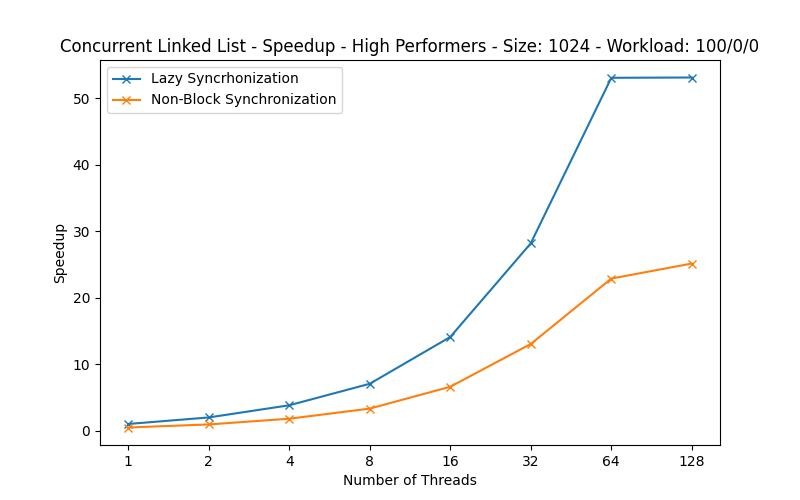
\includegraphics[scale=0.4]{outFiles/plots/concurrent_data_structs_high_speedup_1024_100_0_0.jpg}
        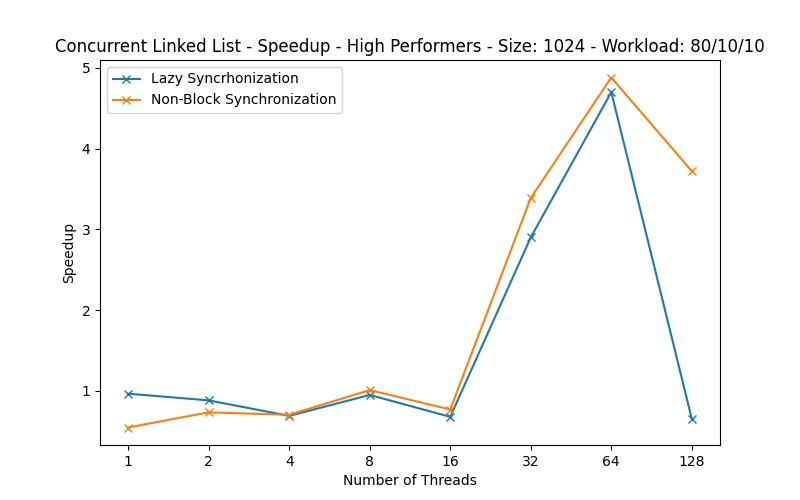
\includegraphics[scale=0.4]{outFiles/plots/concurrent_data_structs_high_speedup_1024_80_10_10.jpg}
        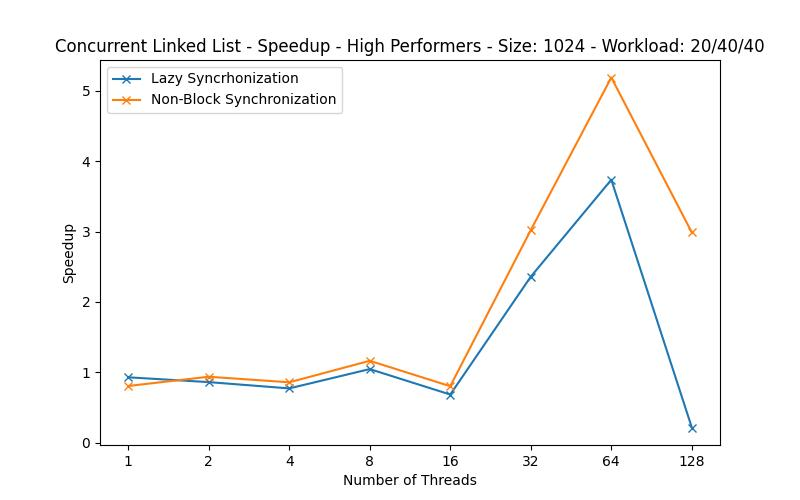
\includegraphics[scale=0.4]{outFiles/plots/concurrent_data_structs_high_speedup_1024_20_40_40.jpg}
        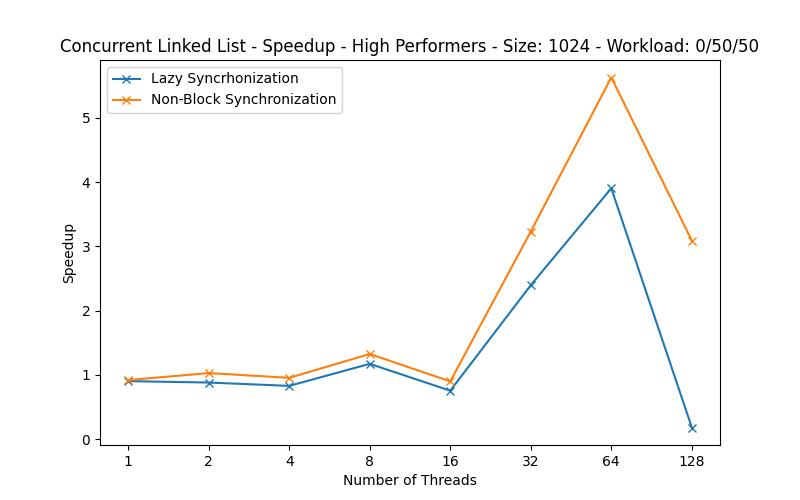
\includegraphics[scale=0.4]{outFiles/plots/concurrent_data_structs_high_speedup_1024_0_50_50.jpg}
    \caption{Concurrent Linked List - Speedup - Size 1024 - High Performers}
    \label{fig:Concurrent Linked List - Speedup - Size 1024 - High Performers}
\end{figure}

\begin{figure}[H]
    \centering
        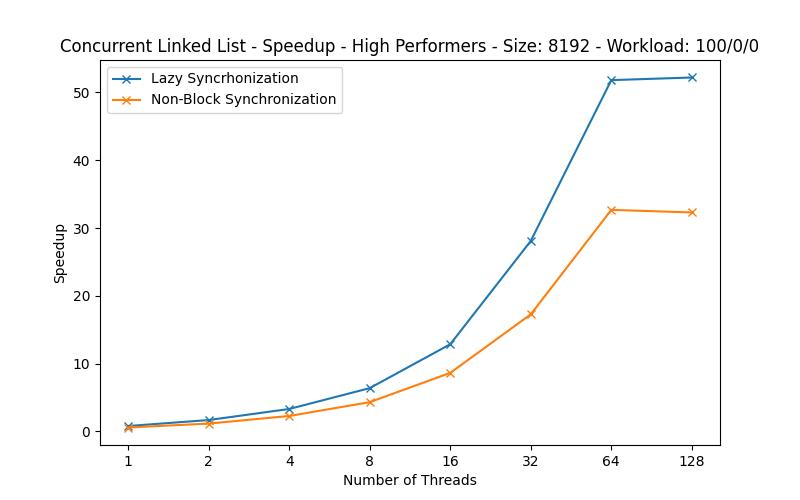
\includegraphics[scale=0.4]{outFiles/plots/concurrent_data_structs_high_speedup_8192_100_0_0.jpg}
        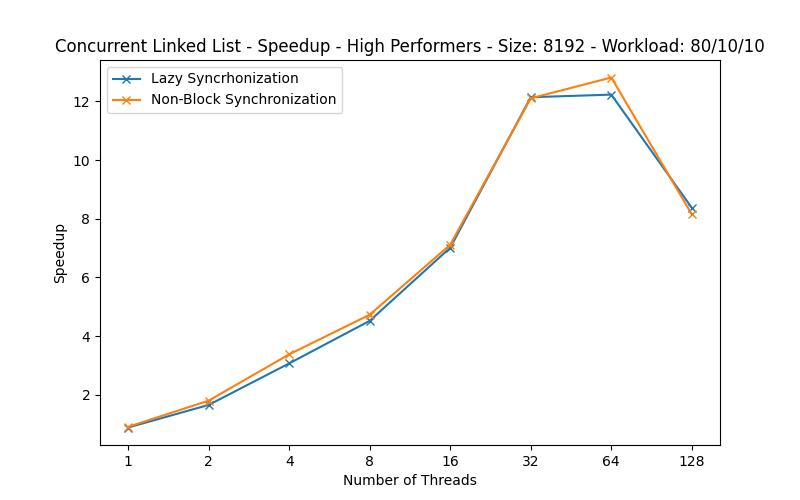
\includegraphics[scale=0.4]{outFiles/plots/concurrent_data_structs_high_speedup_8192_80_10_10.jpg}
        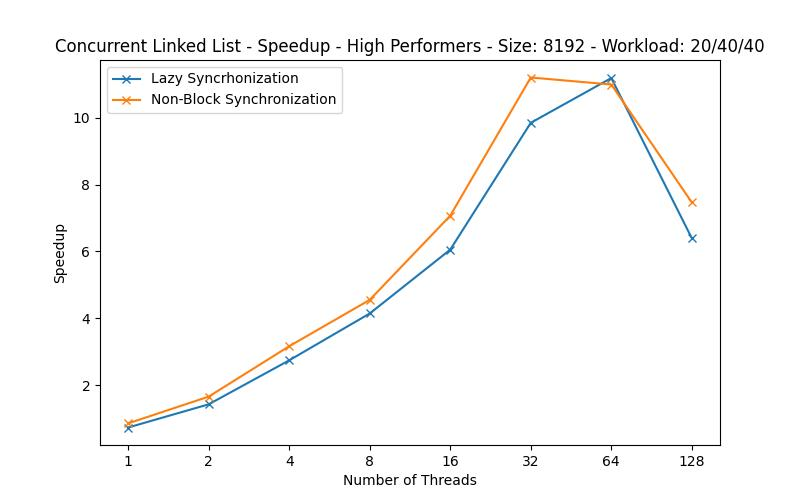
\includegraphics[scale=0.4]{outFiles/plots/concurrent_data_structs_high_speedup_8192_20_40_40.jpg}
        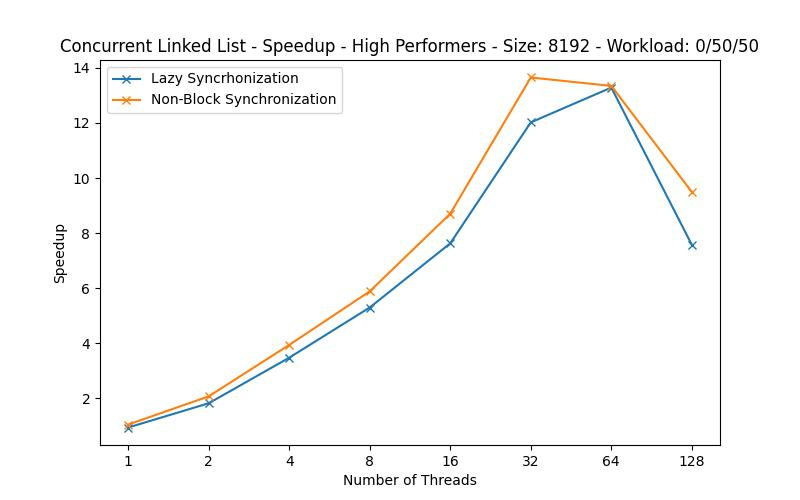
\includegraphics[scale=0.4]{outFiles/plots/concurrent_data_structs_high_speedup_8192_0_50_50.jpg}
    \caption{Concurrent Linked List - Speedup - Size 8192 - High Performers}
    \label{fig:Concurrent Linked List - Speedup - Size 8192 - High Performers}
\end{figure}

\subsection*{High Performers - Συμπεράσματα}
\subsubsection*{Workload}
Για το πρώτο workload που αποτελείται μόνο από contains(), η κλιμάκωση της υλοποίησης είναι σχεδόν ακριβώς γραμμική
για τα πρώτα 64 νήματα. Οι παράμετροι που μελετάμε αυτό το workload είναι λίγο "υπερβολικά ιδανικοί" καθώς δεν υπάρχουν
marked κόμβοι στο πρόβλημα. Αν και οι μέθοδοι contains() είναι ολόιδοι στην θεωρία, στις συγκεκριμένες υλοποιήσεις η non-block
εκδοχή ελέγχει και αν ο δεξιά κόμβος είναι marked ή όχι. Αυτός ο έξτρα έλεγχος που κάνει ευθύνεται και για την μεγάλη διαφορά που
έχουν στο throughput αυτές οι 2 εκδοχές στα περισσότερα νήματα. Το μέγιστο speedup είναι 55 για την lazy και 26 για την non-blocking.

Για τα υπόλοιπα workloads που περιέχουν και add()/remove(), τα αποτελέσματα είναι πάλι αρκετά κοντά μεταξύ τους. Για την μεγάλη λίστα,
οι 2 εκδοχές είναι πρακτικά πανομοιότυπες. Μέχρι τα 16 νήματα, η απόδοση είναι κοντά στην σειριακή. Αυξάνοντας περαιτέρω τα νήματα, το 
throughput τον λιστών "εκτοξεύεται" απευθείας, διπλασιάζοντας με κάθε περαιτέρω διπλασιασμό των νημάτων. Αυτό ισχύει μέχρι τα 128 νήματα
που καταρέει η απόδοση αφού δεν μπορεί να προσφέρει άλλους πυρήνες το σύστημα. Πρέπει πλέον να δρομολογούνται 128 λογικά νήματα σε 64 φυσικά
νήματα. Αυτό το έξτρα overhead καταστρέφει την απόδοση, ειδικά για την lazy λίστα αφού θα αυξάνονται και τα conflicts για απόκτηση των
κλειδαριών. 

\textbf{Σημείωση}: Αν και στην θεωρία η μέθοδος contains() δεν καθαρίζει κόμβους στην non-blocking λίστα, στην υλοποίηση που μας δίνεται
αυτό δεν ισχύει. Η συνάρτηση list\_search είναι κοινή και για τις 3 μεθόδους και εκτελεί έλεγχο για καθαρισμό marked κόμβων.

\subsubsection*{Size}
Το μέγεθος της λίστας έχει αρκετά σημαντικό ρόλο στην απόδοση καθώς μεγαλύτερη λίστα σημαίνει λιγότερα conflicts, τουλάχιστον για τις συγκεκριμένες
λίστες αφού η διάσχιση είναι wait-free. Για μικρές λίστες, η non-blocking λίστα έχει ένα προβάδισμα στην απόδοση ενώ στην μεγαλύτερη λίστα, είναι
πολύ κοντά οι αποδόσεις. Το μικρό αυτό προβάδισμα το αποκτάει η non-blocking καθώς η lazy λίστα έχει ακόμα το ζήτημα των lock conflict. Το φαινόμενο αυτό
είναι πολύ πιο σπάνιο στην μεγάλη λίστα.

Αν και η lazy λίστα έχει το overhead του κλειδώματος, η non-blocking λίστα έχει το 
overhead του compare-and-set. Η lazy λίστα δεν καθιστά σίγουρη την πρόοδο των νημάτων καθώς οι μέθοδοι add() και remove() είναι
τύπου blocking αλλά δεν απαιτεί από κάθε κόμβο να έχει ατομική αναφορά ή να κάνει ατομικό έλεγχο μεταβλητών που "κοστίζει" σε απόδοση.
Περαιτέρω, η non-blocking λίστα απαιτεί να κάνει έλεγχο και διαγραφή των marked κόμβων όσο διατρέχει την λίστα, ενέργεια που μπορεί να
προκαλέσει conflict μεταξύ νημάτων και να αναγκάσει restart της διαδικασίας.

\begin{figure}[H]
    \centering
        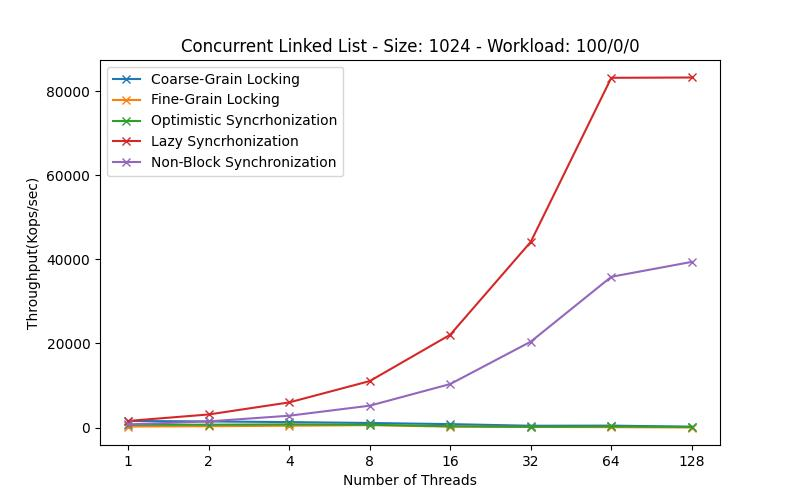
\includegraphics[scale=0.4]{outFiles/plots/concurrent_data_structs_all_1024_100_0_0.jpg}
        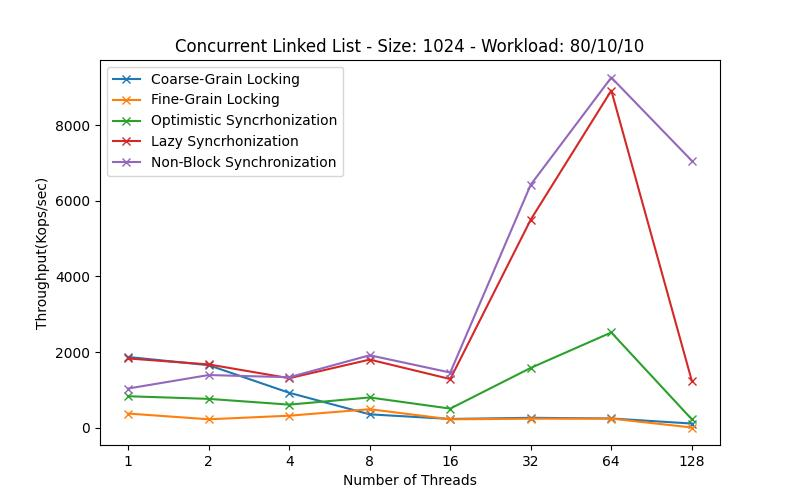
\includegraphics[scale=0.4]{outFiles/plots/concurrent_data_structs_all_1024_80_10_10.jpg}
        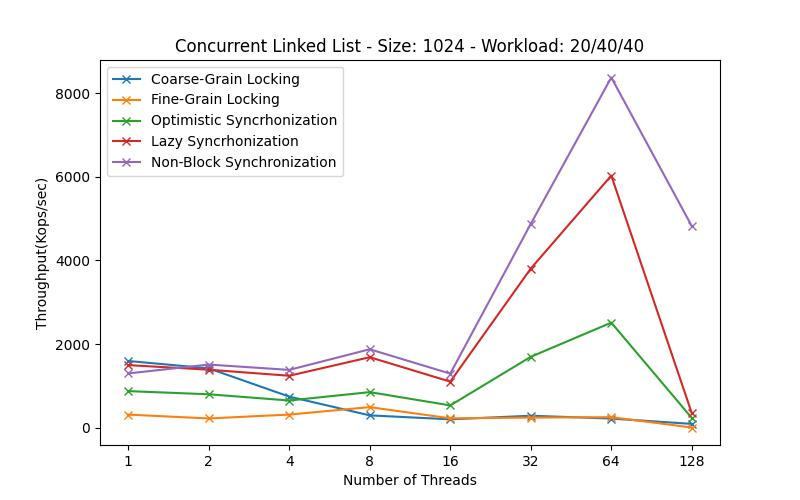
\includegraphics[scale=0.4]{outFiles/plots/concurrent_data_structs_all_1024_20_40_40.jpg}
        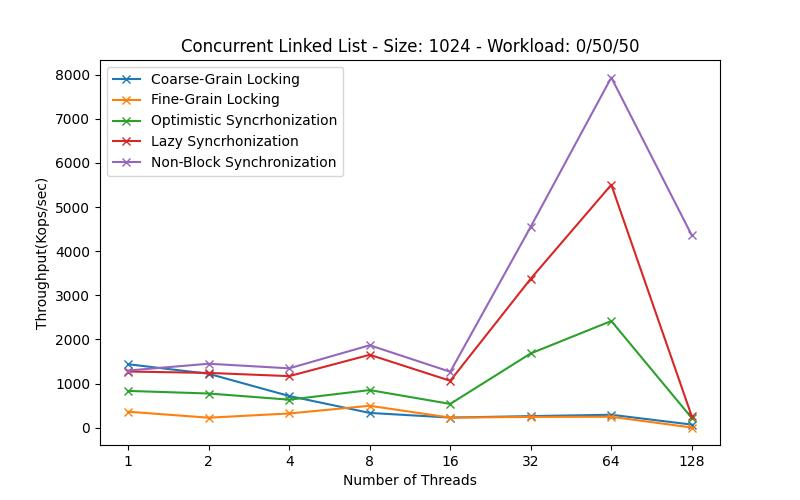
\includegraphics[scale=0.4]{outFiles/plots/concurrent_data_structs_all_1024_0_50_50.jpg}
    \caption{Concurrent Linked List - Throughput - Size 1024 - All Synchronization Techniques}
    \label{fig:Concurrent Linked List - Throughput - Size 1024 - All Synchronization Techniques}
\end{figure}

\begin{figure}[H]
    \centering
        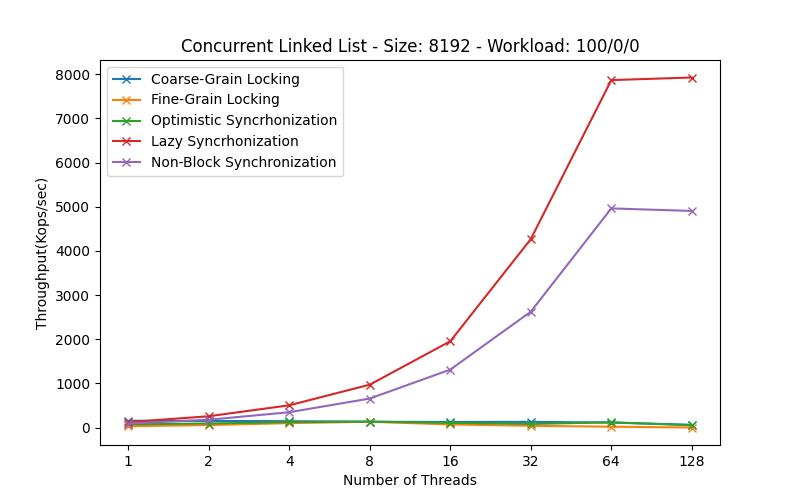
\includegraphics[scale=0.4]{outFiles/plots/concurrent_data_structs_all_8192_100_0_0.jpg}
        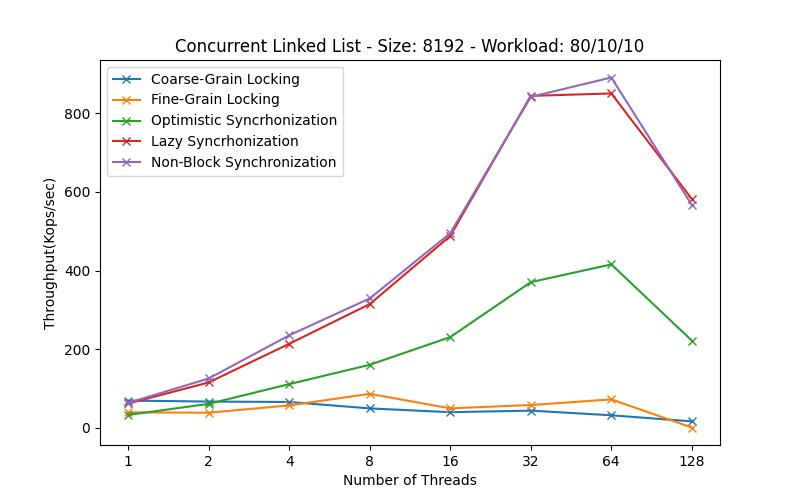
\includegraphics[scale=0.4]{outFiles/plots/concurrent_data_structs_all_8192_80_10_10.jpg}
        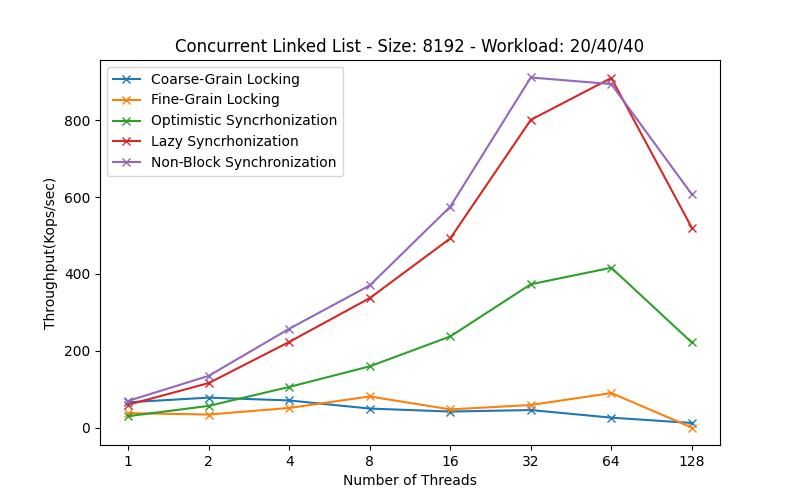
\includegraphics[scale=0.4]{outFiles/plots/concurrent_data_structs_all_8192_20_40_40.jpg}
        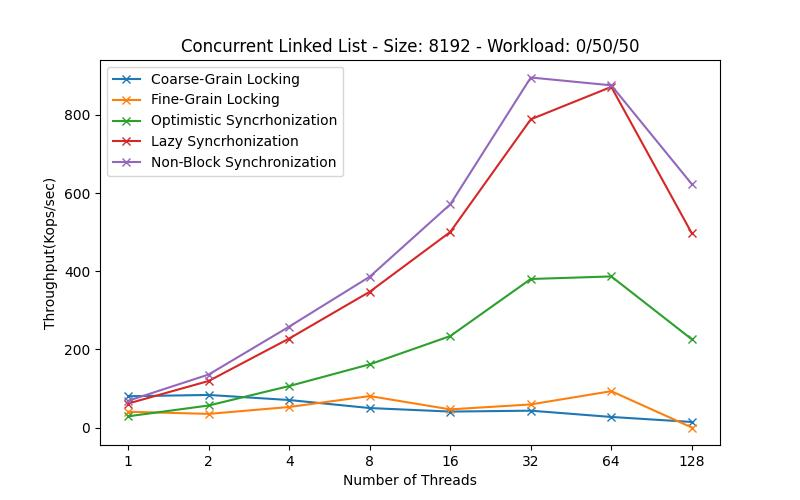
\includegraphics[scale=0.4]{outFiles/plots/concurrent_data_structs_all_8192_0_50_50.jpg}
    \caption{Concurrent Linked List - Throughput - Size 8192 - All Synchronization Techniques}
    \label{fig:Concurrent Linked List - Throughput - Size 8192 - All Synchronization Techniques}
\end{figure}

\begin{figure}[H]
    \centering
        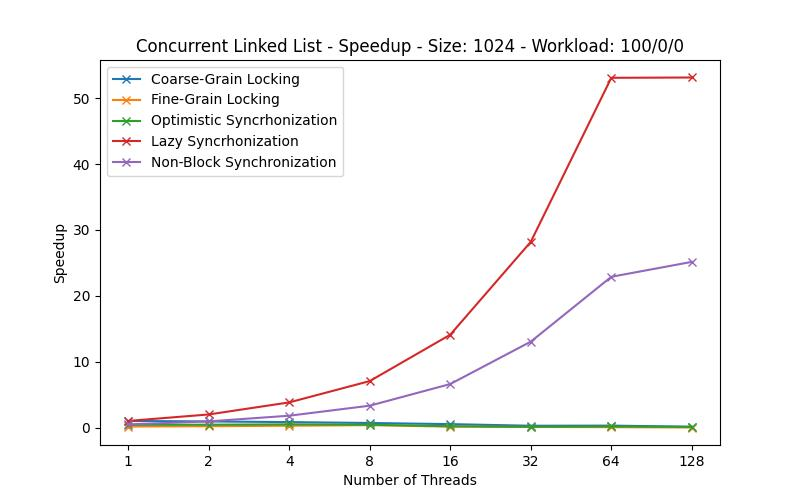
\includegraphics[scale=0.4]{outFiles/plots/concurrent_data_structs_all_speedup_1024_100_0_0.jpg}
        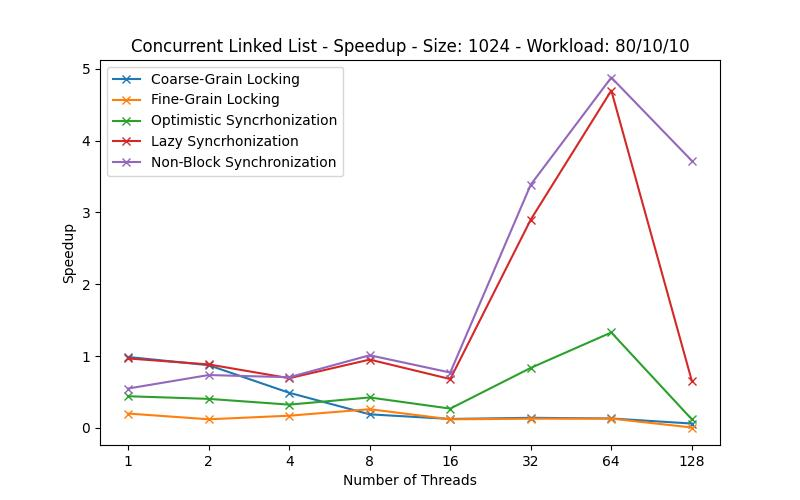
\includegraphics[scale=0.4]{outFiles/plots/concurrent_data_structs_all_speedup_1024_80_10_10.jpg}
        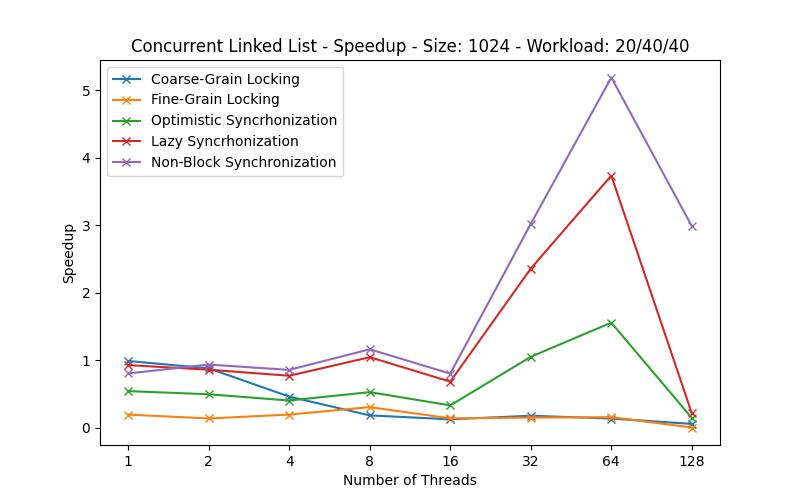
\includegraphics[scale=0.4]{outFiles/plots/concurrent_data_structs_all_speedup_1024_20_40_40.jpg}
        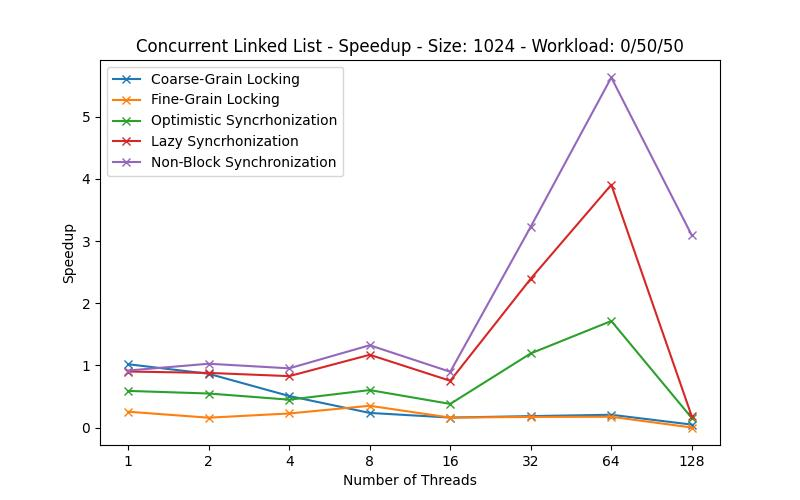
\includegraphics[scale=0.4]{outFiles/plots/concurrent_data_structs_all_speedup_1024_0_50_50.jpg}
    \caption{Concurrent Linked List - Speedup - Size 1024 - All Synchronization Techniques}
    \label{fig:Concurrent Linked List - Speedup - Size 1024 - All Synchronization Techniques}
\end{figure}

\begin{figure}[H]
    \centering
        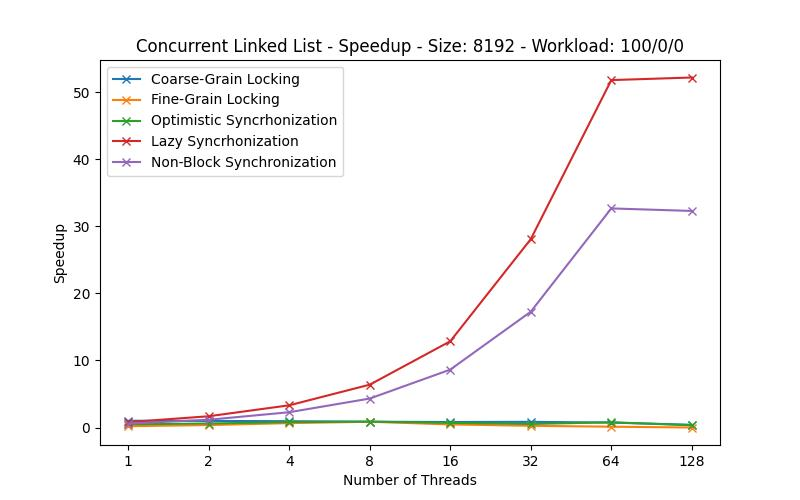
\includegraphics[scale=0.4]{outFiles/plots/concurrent_data_structs_all_speedup_8192_100_0_0.jpg}
        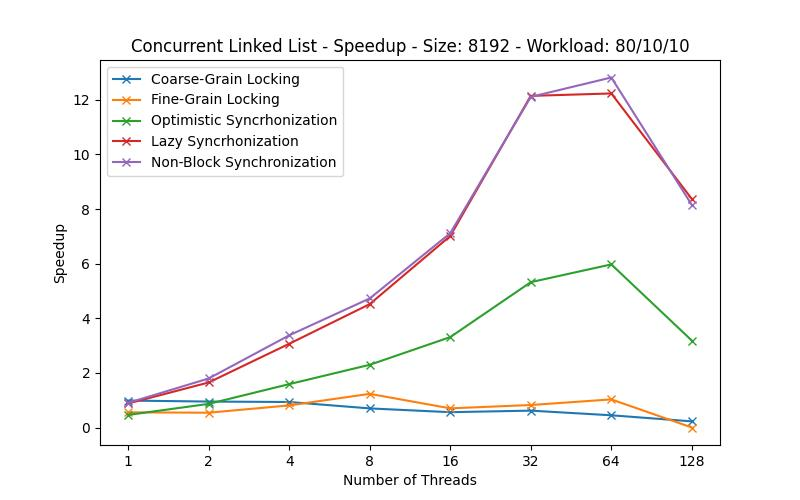
\includegraphics[scale=0.4]{outFiles/plots/concurrent_data_structs_all_speedup_8192_80_10_10.jpg}
        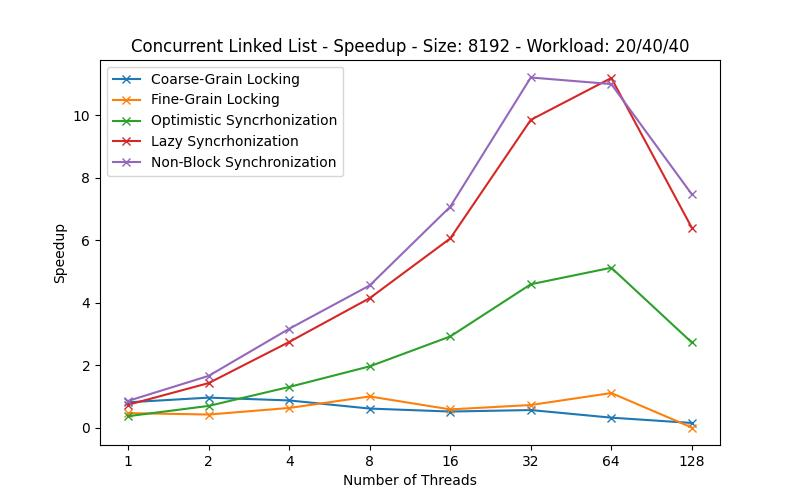
\includegraphics[scale=0.4]{outFiles/plots/concurrent_data_structs_all_speedup_8192_20_40_40.jpg}
        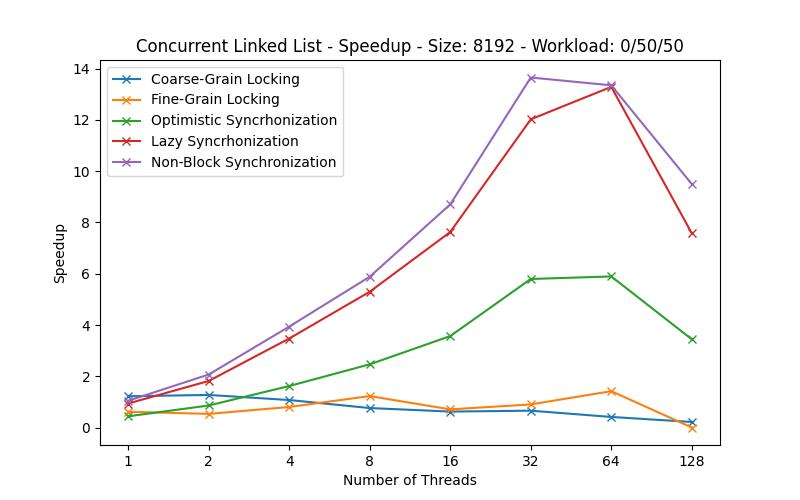
\includegraphics[scale=0.4]{outFiles/plots/concurrent_data_structs_all_speedup_8192_0_50_50.jpg}
    \caption{Concurrent Linked List - Speedup - Size 8192 - All Synchronization Techniques}
    \label{fig:Concurrent Linked List - Speedup - Size 8192 - All Synchronization Techniques}
\end{figure}

\subsection*{Τελικά Συμπεράσματα}
Οι coarse-grained, fine-grained και optimistic synchronization λίστες έχουν αρκετά θεωρητικά προβλήματα που παρουσιάζονται
και στα αποτελέσματα των πειραμάτων. Οι δύο πρώτες δεν καταφέρνουν να ξεπεράσουν τις επιδόσεις της σειριακής δομής ενώ η τρίτη
έχει μέτριες επιδόσεις, ειδικά σε μικρές λίστες. Σε μεγάλες λίστες, τα συμπεράσματα είναι λίγο διαφορετικά για την optimistic λίστα, με
κάποιες μικρές προοπτικές για κλιμάκωση.

Σε αντίθεση, η lazy και η non-blocking λίστα είναι πιο εκλεπτυσμένες λύσεις.
Δεν μπορούμε να πούμε ότι η non-blocking είναι βελτίωση της lazy καθώς η μία μπορεί να αντικαταστήσει την άλλη, αναλόγως την εφαρμογή.
Η non-blocking είναι robust λύση χωρίς locks αλλά με μεγαλύτερο performance drawback λόγω των συνεχόμενων compare-and-set. Αντιθέτως, η
lazy έχει locks στις μεθόδους add()/remove() όμως είναι πιο γρήγορη σε workload που αποτελούνται μόνο από contains().

\textbf{Σημείωση}: Πιστεύουμε ότι και η non-blocking θα είχε ίδια απόδοση με την lazy στο 100/0/0 workload αν δεν αναγκάζοταν να διαγράφει
τα marked nodes, όπως κάνει στην δοσμένη υλοποίηση.

`='